\documentclass[11pt]{article}
\usepackage[margin=1in]{geometry}
\usepackage{amsmath,amssymb,amsthm}
\usepackage{mathtools}
\usepackage{tikz}
\usepackage{booktabs}
\usepackage{array}
\usepackage{enumitem}
\usepackage{xcolor}
\usepackage{fancyhdr}
\usepackage{titlesec}
\usepackage{hyperref}

\hypersetup{colorlinks=true, linkcolor=blue, urlcolor=blue}

\titleformat{\section}{\normalfont\Large\bfseries}{}{0em}{}
\titlespacing*{\section}{0pt}{1.5em}{1em}
\renewcommand{\thesection}{\arabic{section}}

\setlength{\headheight}{14pt}
\pagestyle{fancy}
\fancyhf{}
\fancyhead[L]{APM1220: FA 2 --- Sample Geometry and Random Sampling}
\fancyhead[R]{\thepage}
\renewcommand{\headrulewidth}{0.4pt}

\newcommand{\bx}{\mathbf{x}}
\newcommand{\by}{\mathbf{y}}
\newcommand{\bX}{\mathbf{X}}
\newcommand{\bS}{\mathbf{S}}
\newcommand{\ba}{\mathbf{a}}
\newcommand{\bd}{\mathbf{d}}
\newcommand{\bD}{\mathbf{D}}
\newcommand{\bR}{\mathbf{R}}
\newcommand{\one}{\mathbf{1}}

\newenvironment{sol}{\par\noindent\textbf{Solution.}\quad}{\par\medskip}

\title{\vspace{-2cm}APM1220: Applied Multivariate Data Analysis \\[4pt]
\large FA 2. Sample Geometry and Random Sampling}
\author{}
\date{}

\begin{document}
\maketitle
\thispagestyle{fancy}
\vspace{-1.5cm}

\section{Problem 3.1 (8 points)}

Given the data matrix
\[
\bX = \begin{pmatrix} 9 & 1 \\ 5 & 3 \\ 1 & 2 \end{pmatrix}, \qquad n=3,\; p=2.
\]

The column means are
\[
\bar x_1 = \frac{9+5+1}{3} = 5, \qquad \bar x_2 = \frac{1+3+2}{3} = 2, \qquad \bar\bx' = (5,\,2).
\]

\subsection*{(a) Scatter plot in $p=2$ dimensions}

\begin{sol}
\begin{center}
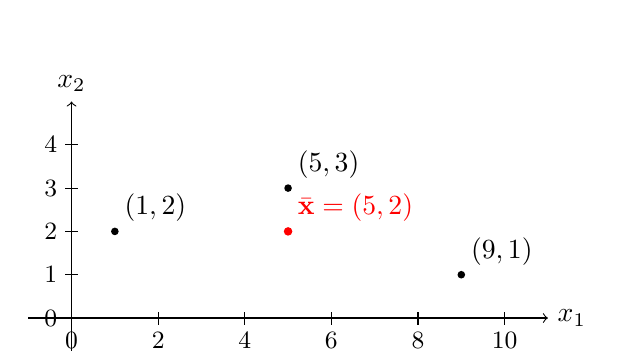
\begin{tikzpicture}[scale=0.55]
\draw[->] (-1,0) -- (11,0) node[right]{$x_1$};
\draw[->] (0,-1) -- (0,5) node[above]{$x_2$};
\foreach \x in {0,2,4,6,8,10} \draw (\x,-0.15) -- (\x,0.15) node[below=4pt]{\small \x};
\foreach \y in {0,1,2,3,4} \draw (-0.15,\y) -- (0.15,\y) node[left=4pt]{\small \y};
\fill (9,1) circle (2.5pt) node[above right]{$(9,1)$};
\fill (5,3) circle (2.5pt) node[above right]{$(5,3)$};
\fill (1,2) circle (2.5pt) node[above right]{$(1,2)$};
\fill[red] (5,2) circle (2.8pt) node[above right, red]{$\bar\bx=(5,2)$};
\end{tikzpicture}
\end{center}
The three observations $(9,1)$, $(5,3)$, $(1,2)$ are plotted in the $x_1$-$x_2$ plane, along with the sample mean point $\bar\bx=(5,2)$, which lies at the centroid of the three points.
\end{sol}

\subsection*{(b) $n$-dimensional representation and deviation vectors}

\begin{sol}
Each \emph{variable} (column of $\bX$) is now viewed as a vector in $n=3$-dimensional space:
\[
\by_1 = \begin{pmatrix}9\\5\\1\end{pmatrix}, \qquad \by_2 = \begin{pmatrix}1\\3\\2\end{pmatrix}.
\]
The deviation vectors are obtained by subtracting the corresponding sample mean (times $\one$) from each column:
\[
\by_1 - \bar x_1\one = \begin{pmatrix}9\\5\\1\end{pmatrix} - 5\begin{pmatrix}1\\1\\1\end{pmatrix} = \begin{pmatrix}4\\0\\-4\end{pmatrix} =: \bd_1,
\]
\[
\by_2 - \bar x_2\one = \begin{pmatrix}1\\3\\2\end{pmatrix} - 2\begin{pmatrix}1\\1\\1\end{pmatrix} = \begin{pmatrix}-1\\1\\0\end{pmatrix} =: \bd_2.
\]

Conceptually, $\by_1$ and $\by_2$ are vectors from the origin to the points $(9,5,1)$ and $(1,3,2)$ in $\mathbb{R}^3$; the deviation vectors $\bd_1=\by_1-\bar x_1\one$ and $\bd_2=\by_2-\bar x_2\one$ are the components of $\by_1,\by_2$ that are \emph{perpendicular} to the equiangular line $\one=(1,1,1)'$ (since each $\bd_i$ sums to zero).
\end{sol}

\subsection*{(c) Deviation vectors from the origin: lengths, angle, and connection to $\bS_n$ and $\bR$}

\begin{sol}
\begin{center}
\begin{tikzpicture}[scale=0.85]
\draw[->,thick,blue] (0,0) -- (4,0) node[right]{$\bd_1=(4,0,-4)'$};
\draw[->,thick,red] (0,0) -- (-1.4,1.6) node[above]{$\bd_2=(-1,1,0)'$};
\fill (0,0) circle (1.5pt) node[below left]{$O$};
\draw (0.9,0) arc (0:131:0.9);
\node at (0.2,0.55) {\small $\theta$};
\end{tikzpicture}
\end{center}
(Sketch shown in a convenient 2-D projection since both vectors, together with the origin, span a plane; the true angle between them in $\mathbb{R}^3$ is computed below.)

\textbf{Lengths:}
\[
L_1 = |\bd_1| = \sqrt{4^2+0^2+(-4)^2} = \sqrt{32} = 4\sqrt{2}, \qquad
L_2 = |\bd_2| = \sqrt{(-1)^2+1^2+0^2} = \sqrt{2}.
\]

\textbf{Cosine of the angle between $\bd_1$ and $\bd_2$:}
\[
\bd_1'\bd_2 = (4)(-1)+(0)(1)+(-4)(0) = -4,
\]
\[
\cos\theta = \frac{\bd_1'\bd_2}{L_1 L_2} = \frac{-4}{(4\sqrt{2})(\sqrt{2})} = \frac{-4}{8} = -\frac12
\qquad\Longrightarrow\qquad \theta = 120^\circ.
\]

\textbf{Connection to $\bS_n$ and $\bR$.} With the divisor-$n$ covariance matrix $\bS_n$ ($s_{ii}=\bd_i'\bd_i/n$, $s_{ij}=\bd_i'\bd_j/n$):
\[
s_{11} = \frac{L_1^2}{n} = \frac{32}{3}, \qquad s_{22} = \frac{L_2^2}{n} = \frac{2}{3}, \qquad
s_{12} = \frac{\bd_1'\bd_2}{n} = \frac{-4}{3}.
\]
The sample correlation coefficient is
\[
r_{12} = \frac{s_{12}}{\sqrt{s_{11}s_{22}}} = \frac{-4/3}{\sqrt{(32/3)(2/3)}} = \frac{-4/3}{8/3} = -\frac12 = \cos\theta.
\]
This confirms the general geometric fact: \emph{the cosine of the angle between the two deviation vectors equals the sample correlation coefficient $r_{12}$ between the two variables}, and the squared lengths of the deviation vectors are proportional ($\times n$) to the sample variances $s_{11}$ and $s_{22}$.
\end{sol}

\clearpage
\section{Problem 3.6 (8 points)}

\[
\bX = \begin{pmatrix} -1 & 3 & -2 \\ 2 & 4 & 2 \\ 5 & 2 & 3\end{pmatrix}, \qquad n=3,\; p=3.
\]

\subsection*{(a) Matrix of deviations $\bX-\one\bar\bx'$ and its rank}

\begin{sol}
Column means:
\[
\bar x_1 = \frac{-1+2+5}{3}=2, \quad \bar x_2=\frac{3+4+2}{3}=3, \quad \bar x_3 = \frac{-2+2+3}{3}=1, \qquad \bar\bx'=(2,3,1).
\]
\[
\bX - \one\bar\bx' =
\begin{pmatrix}-1-2 & 3-3 & -2-1\\ 2-2 & 4-3 & 2-1 \\ 5-2 & 2-3 & 3-1\end{pmatrix}
= \begin{pmatrix} -3 & 0 & -3 \\ 0 & 1 & 1 \\ 3 & -1 & 2\end{pmatrix} =: \bD.
\]
Its determinant is
\[
\det(\bD) = -3(1\cdot2 - 1\cdot(-1)) - 0(0\cdot2-1\cdot3) + (-3)(0\cdot(-1)-1\cdot3) = -3(3) -0 + (-3)(-3) = -9+9=0.
\]
Since $\det(\bD)=0$, $\bD$ is \textbf{not of full rank} (rank $<3$). This is expected: because each column of a mean-corrected data matrix sums to zero, every column of $\bD$ lies in the $(n-1)$-dimensional subspace of $\mathbb{R}^n$ orthogonal to $\one$. With $n=3$, this subspace has dimension $2$, so the $p=3$ column vectors of $\bD$ (each in $\mathbb{R}^3$) cannot be linearly independent — at most $\operatorname{rank}(\bD)=\min(p,n-1)=2$.
\end{sol}

\subsection*{(b) Sample covariance matrix $\bS$ and generalized variance $|\bS|$}

\begin{sol}
$\bS = \dfrac{1}{n-1}\bD'\bD = \dfrac12 \bD'\bD$. Writing the columns of $\bD$ as $\bd_1=(-3,0,3)'$, $\bd_2=(0,1,-1)'$, $\bd_3=(-3,1,2)'$:
\[
\bD'\bD = \begin{pmatrix} 18 & -3 & 15\\ -3 & 2 & -1 \\ 15 & -1 & 14\end{pmatrix}, \qquad
\bS = \frac12\begin{pmatrix} 18 & -3 & 15\\ -3 & 2 & -1 \\ 15 & -1 & 14\end{pmatrix}
= \begin{pmatrix} 9 & -\dfrac32 & \dfrac{15}{2} \\[4pt] -\dfrac32 & 1 & -\dfrac12 \\[4pt] \dfrac{15}{2} & -\dfrac12 & 7\end{pmatrix}.
\]
Because $\bD$ has rank $2<3$, $\bD'\bD$ (and hence $\bS$) is \textbf{singular}:
\[
|\bS| = 0.
\]
\textbf{Geometric interpretation.} The generalized sample variance $|\bS|$ is proportional to the squared volume of the parallelotope spanned by the $p=3$ deviation vectors $\bd_1,\bd_2,\bd_3$ in $n$-space (specifically $|\bS|=\text{vol}^2/(n-1)^p$). Since $|\bS|=0$, this parallelotope has \textbf{zero volume}: the three deviation vectors are linearly dependent and therefore all lie in a common plane (a 2-dimensional subspace) rather than spanning a genuine 3-dimensional solid. Equivalently, the scatter of the $n=3$ points does not "fill up" all $p=3$ dimensions — one variable is redundant given the other two.
\end{sol}

\subsection*{(c) Total sample variance}

\begin{sol}
The total sample variance is the trace of $\bS$ (sum of the sample variances of the individual variables):
\[
\operatorname{tr}(\bS) = s_{11}+s_{22}+s_{33} = 9 + 1 + 7 = \boxed{17}.
\]
\end{sol}

\clearpage
\section{Problem 3.9 (8 points)}

\[
\bX = \begin{pmatrix} 12 & 17 & 29\\ 18 & 20 & 38 \\ 14 & 16 & 30 \\ 20 & 18 & 38 \\ 16 & 19 & 35\end{pmatrix}, \qquad n=5,
\]
where $x_3 = x_1+x_2$ (total of the two tests).

\subsection*{(a) Mean-corrected data matrix and linear dependence}

\begin{sol}
Column means:
\[
\bar x_1 = \frac{12+18+14+20+16}{5}=16,\qquad \bar x_2 = \frac{17+20+16+18+19}{5}=18,
\]
\[
\bar x_3=\frac{29+38+30+38+35}{5}=34.
\]
Note $\bar x_1+\bar x_2 = 34 = \bar x_3$, as expected. The mean-corrected matrix is
\[
\bX - \one\bar\bx' =
\begin{pmatrix} -4 & -1 & -5\\ 2 & 2 & 4\\ -2 & -2 & -4\\ 4 & 0 & 4\\ 0 & 1 & 1\end{pmatrix}=:\bD.
\]
Column 3 of $\bD$ equals the sum of columns 1 and 2 in every row:
\[
(-4)+(-1)=-5,\quad 2+2=4,\quad(-2)+(-2)=-4,\quad 4+0=4,\quad 0+1=1.
\]
Hence the columns are linearly dependent, with
\[
\ba' = (a_1,a_2,a_3) = (1,\,1,\,-1), \qquad \text{since } a_1\bd_1+a_2\bd_2+a_3\bd_3 = \mathbf 0.
\]
\end{sol}

\subsection*{(b) Sample covariance matrix, $|\bS|=0$, and $\bS\ba=\mathbf 0$}

\begin{sol}
With $\bd_1=(-4,2,-2,4,0)'$, $\bd_2=(-1,2,-2,0,1)'$, $\bd_3=(-5,4,-4,4,1)'$ and $n-1=4$:
\[
\bD'\bD = \begin{pmatrix} 40 & 12 & 52 \\ 12 & 10 & 22 \\ 52 & 22 & 74\end{pmatrix}, \qquad
\bS = \frac14\bD'\bD = \begin{pmatrix} 10 & 3 & 13 \\ 3 & \dfrac52 & \dfrac{11}{2} \\ 13 & \dfrac{11}{2} & \dfrac{37}{2}\end{pmatrix}.
\]
Because $\bd_3=\bd_1+\bd_2$, the columns of $\bD$ are linearly dependent (rank $\bD\le2<3$), so $\bS$ is singular and
\[
|\bS| = 0.
\]
\textbf{Verification that $\bS\ba=\mathbf 0$} for $\ba=(1,1,-1)'$:
\[
\bS\ba = \begin{pmatrix} 10(1)+3(1)+13(-1) \\ 3(1)+\tfrac52(1)+\tfrac{11}{2}(-1) \\ 13(1)+\tfrac{11}{2}(1)+\tfrac{37}{2}(-1)\end{pmatrix}
= \begin{pmatrix} 10+3-13 \\ 3+2.5-5.5 \\ 13+5.5-18.5\end{pmatrix}
= \begin{pmatrix}0\\0\\0\end{pmatrix}.
\]
Since $\bS\ba = 0\cdot\ba$, the vector $\ba=(1,1,-1)'$ (or any nonzero scalar multiple of it) is an eigenvector of $\bS$ corresponding to the eigenvalue $\lambda=0$.
\end{sol}

\subsection*{(c) Verifying $x_3 = x_1+x_2$}

\begin{sol}
Checking each row of $\bX$ directly:
\[
12+17=29,\quad 18+20=38,\quad 14+16=30,\quad 20+18=38,\quad 16+19=35,
\]
each of which matches the corresponding entry of column 3. Hence for every observation,
\[
x_1 + x_2 - x_3 = 0 \quad\Longleftrightarrow\quad a_1 x_1+a_2x_2+a_3x_3=0 \text{ with } a_1=1,\ a_2=1,\ a_3=-1,
\]
confirming the exact linear dependence among the three columns (as used in parts (a) and (b)).
\end{sol}

\clearpage
\section{Problem 3.18 (8 points)}

Summary statistics for 2001 state energy consumption ($x_1$ = petroleum, $x_2$ = natural gas, $x_3$ = hydroelectric, $x_4$ = nuclear; quadrillion BTUs):
\[
\bar\bx = \begin{pmatrix}0.766\\0.508\\0.438\\0.161\end{pmatrix}, \qquad
\bS = \begin{pmatrix}
0.856 & 0.635 & 0.173 & 0.096\\
0.635 & 0.568 & 0.128 & 0.067\\
0.173 & 0.128 & 0.171 & 0.039\\
0.096 & 0.067 & 0.039 & 0.043
\end{pmatrix}.
\]
(The off-diagonal entry $s_{23}=s_{32}$ is taken as $0.128$, the symmetric value, to correct a printing rounding inconsistency in the source table.)

\subsection*{(a) Mean and variance of total energy consumption}

\begin{sol}
Total consumption is the linear combination $T = x_1+x_2+x_3+x_4 = \mathbf{c}'\bx$ with $\mathbf{c}=(1,1,1,1)'$.

\textbf{Mean:}
\[
\bar T = \mathbf{c}'\bar\bx = 0.766+0.508+0.438+0.161 = 1.873 \text{ (quadrillion BTUs)}.
\]

\textbf{Variance:} $\operatorname{Var}(T) = \mathbf{c}'\bS\mathbf{c} = \sum_{i}\sum_{j} s_{ij}$, i.e., the sum of \emph{all} entries of $\bS$:
\[
\begin{aligned}
\operatorname{Var}(T) &= (0.856+0.635+0.173+0.096) + (0.635+0.568+0.128+0.067)\\
&\quad + (0.173+0.128+0.171+0.039) + (0.096+0.067+0.039+0.043)\\
&= 1.760 + 1.398 + 0.511 + 0.245 \\
&= \boxed{3.914}.
\end{aligned}
\]
\end{sol}

\subsection*{(b) Excess of petroleum over natural gas; covariance with total}

\begin{sol}
Let $D = x_1-x_2 = \mathbf{b}'\bx$ with $\mathbf{b}=(1,-1,0,0)'$.

\textbf{Mean:}
\[
\bar D = \bar x_1 - \bar x_2 = 0.766-0.508 = 0.258.
\]

\textbf{Variance:}
\[
\operatorname{Var}(D) = \mathbf{b}'\bS\mathbf{b} = s_{11}-2s_{12}+s_{22} = 0.856 - 2(0.635) + 0.568 = 0.154.
\]

\textbf{Covariance of $D$ with $T$ (part a):}
\[
\operatorname{Cov}(D,T) = \mathbf{b}'\bS\mathbf{c} = (s_{11}+s_{12}+s_{13}+s_{14}) - (s_{21}+s_{22}+s_{23}+s_{24}).
\]
Using the row sums already computed in part (a) (row 1 sum $=1.760$, row 2 sum $=1.398$):
\[
\operatorname{Cov}(D,T) = 1.760 - 1.398 = \boxed{0.362}.
\]
\end{sol}

\clearpage
\section{Problem 3.20 (8 points)}

Snow-removal data for $n=25$ Wisconsin storms: $x_1=$ storm duration (hrs), $x_2=$ crew/machine hours to clear snow.

Summary sums (computed directly from Table 3.2):
\[
\sum x_{j1} = 235.5,\qquad \sum x_{j2}=481.8,\qquad \sum x_{j1}^2 = 2557.75,
\]
\[
\sum x_{j2}^2 = 10778.98,\qquad \sum x_{j1}x_{j2}=4861.90.
\]

From these,
\[
\bar x_1 = \frac{235.5}{25}=9.420, \qquad \bar x_2 = \frac{481.8}{25}=19.272,
\]
\[
s_{11} = \frac{\sum x_{j1}^2 - n\bar x_1^2}{n-1} = \frac{2557.75 - 25(9.42)^2}{24} = 14.1392,
\]
\[
s_{22} = \frac{\sum x_{j2}^2 - n\bar x_2^2}{n-1} = \frac{10778.98-25(19.272)^2}{24} = 62.2388,
\]
\[
s_{12} = \frac{\sum x_{j1}x_{j2}-n\bar x_1\bar x_2}{n-1} = \frac{4861.90-25(9.42)(19.272)}{24} = 13.4727.
\]

\subsection*{(a) Mean and variance of $x_2-x_1$ from the summary statistics}

\begin{sol}
\textbf{Mean:}
\[
\overline{x_2-x_1} = \bar x_2-\bar x_1 = 19.272-9.420 = 9.852.
\]
\textbf{Variance:}
\[
\operatorname{Var}(x_2-x_1) = s_{11}+s_{22}-2s_{12} = 14.1392+62.2388-2(13.4727) = \boxed{49.4326}.
\]
\end{sol}

\subsection*{(b) Mean and variance from the individual differences $d_j = x_{j2}-x_{j1}$}

\begin{sol}
Computing $d_j = x_{j2}-x_{j1}$ for each $j=1,\dots,25$ and summing:
\[
\sum_{j=1}^{25} d_j = 246.3, \qquad \sum_{j=1}^{25} d_j^2 = 3612.93.
\]
\textbf{Mean:}
\[
\bar d = \frac{246.3}{25} = 9.852.
\]
\textbf{Variance:}
\[
s_d^2 = \frac{\sum d_j^2 - n\bar d^2}{n-1} = \frac{3612.93 - 25(9.852)^2}{24} = \frac{3612.93-2426.567}{24}=\frac{1186.363}{24} = \boxed{49.4326}.
\]

\textbf{Comparison.} The mean ($9.852$) and variance ($49.4326$) obtained by first computing individual differences $d_j$ and then their sample mean/variance are \textbf{identical} to those obtained in part (a) using the summary statistics $\bar x_1,\bar x_2,s_{11},s_{22},s_{12}$. This confirms the general algebraic identities
\[
\overline{x_2-x_1} = \bar x_2 - \bar x_1, \qquad \operatorname{Var}(x_2-x_1)=s_{11}+s_{22}-2s_{12},
\]
which hold exactly for any bivariate sample, so the two computational routes must agree.
\end{sol}

\end{document}
